\documentclass[aspectratio=169]{beamer}
\usetheme{Madrid}
\usecolortheme{default}
\usepackage{tikz}
\usetikzlibrary{calc,shapes,arrows.meta,positioning}

% --- Organization slides (TOC + section dividers) ---
\AtBeginSection[]
{
  \begin{frame}{Outline}
    \tableofcontents[currentsection]
  \end{frame}
}

\title{Lecture 3: Improving Performance}
\subtitle{Context Engineering Techniques for Better Results}
\author{University of Chicago}
\date{\today}

\begin{document}

\frame{\titlepage}

\section{Where We Are}

\begin{frame}{Review: What We've Covered}
\textbf{Lecture 1: Foundations}
\begin{itemize}
    \item Basic AI terminology (LLMs, tokens, context windows, APIs)
    \item How to work with these models programmatically
    \item Understanding pricing and token economics
\end{itemize}
\vspace{0.3cm}

\textbf{Lecture 2: Building AI Systems}
\begin{itemize}
    \item Vertical slices - prove end-to-end flow works first
    \item Crawl, Walk, Run - start simple, add complexity incrementally
    \item Breaking problems into clear inputs and outputs
\end{itemize}
\end{frame}

\begin{frame}{Where We're Going}
\textbf{Last Time}: We built a basic resume scoring system
\begin{itemize}
    \item Single prompt: resume + job requirements → 0-100 score
\end{itemize}
\vspace{0.3cm}

\textbf{Today}: Learn techniques to improve AI system performance
\begin{itemize}
    \item \textbf{Lecture}: Walk through a simple example (expense validation)
    \item \textbf{Work Session}: Apply these same techniques to improve the resume scorer
\end{itemize}
\vspace{0.3cm}

\end{frame}

\section{Performance Improvement}

\begin{frame}{The Core Problem}
\textbf{It's difficult to know what does and does not work with AI Systems.}

\begin{itemize}
    \item Results are inconsistent and non-deterministic
    \item Hard to debug when things go wrong
    \item Model hallucinates or makes up information
    \item Edge cases get mishandled
    \item We (often) can't explain \textit{why} the model decided something
\end{itemize}
\vspace{0.3cm}

\textbf{This is why we use vertical slices -- to identify processes that require improvement.}
\end{frame}

\begin{frame}{The Core Problem}
\textbf{Our resume scorer from Lecture 2 had issues:}
\begin{itemize}
    \item Scores ranged from 0-100, but were they \textit{good}?
    \item Results tended to be bunchy (most scores clustered in narrow ranges)
    \item Difficult to interpret what a "65" meant vs. a "75"
    \item No clear explanation for why a candidate got their score
    \item Hard to defend decisions to hiring managers
\end{itemize}
\vspace{0.3cm}

\textbf{How do we make this better?}
\begin{itemize}
    \item Break down what we're measuring
    \item Provide evidence for claims
    \item Make the scoring process more transparent
\end{itemize}
\end{frame}

\begin{frame}{The Core Problem}
\textbf{Solution}: Engineering the context more carefully
\begin{itemize}
	\item How?
\begin{itemize}
    \item Break complex problems into simpler steps
    \item Ground the model with evidence requirements
    \item Provide examples to guide behavior
\end{itemize}
\end{itemize}
\end{frame}

\section{Expense Report System}

\begin{frame}{Expense Report Validator}
\textbf{Task}: Validate employee expense reports for compliance
\vspace{0.3cm}

\textbf{Input}: Receipt/invoice text + description
\vspace{0.2cm}

\textbf{Required Outputs}:
\begin{itemize}
    \item Expense type (Travel, Office Supplies, Meals/Entertainment)
    \item Date and location
    \item Compliance issues
\end{itemize}
\vspace{0.3cm}

\textbf{Compliance Rules}:
\begin{enumerate}
    \item \textbf{Amount limits}: Different limits per category
    \item \textbf{Required fields}: Travel requires trip purpose, Meals require attendees
    \item \textbf{Prohibited expenses}: No alcohol reimbursement
\end{enumerate}
\end{frame}

\begin{frame}{Example 1: Travel Expense}
\begin{columns}[T]
\begin{column}{0.48\textwidth}
\textbf{Receipt}:
\vspace{0.2cm}

{\small\texttt{
\begin{tabular}{l}
Conference Badge \\
AI Summit 2024 \\
Jan 15-17, 2024 \\
San Francisco, CA \\
\\
Registration: \$495.00 \\
Processing Fee: \$15.00 \\
\hline
Total: \$510.00
\end{tabular}
}}
\end{column}

\begin{column}{0.48\textwidth}
\textbf{Expected Output}:
\vspace{0.2cm}

{\small
\begin{itemize}
    \item \textbf{Type}: Travel
    \item \textbf{Date}: Jan 15-17, 2024
    \item \textbf{Location}: San Francisco, CA
    \item \textbf{Amount}: \$510.00
    \item \textbf{Required fields}: Trip purpose (conference), destination
    \item \textbf{Compliance}: Pass
\end{itemize}
}
\end{column}
\end{columns}
\end{frame}

\begin{frame}{Example 2: Meals with Alcohol}
\begin{columns}[T]
\begin{column}{0.48\textwidth}
\textbf{Receipt}:
\vspace{0.2cm}

{\small\texttt{
\begin{tabular}{l}
The Steakhouse \\
Boston, MA \\
Jan 20, 2024 \\
\\
2x Ribeye Steak: \$68.00 \\
1x Caesar Salad: \$14.00 \\
1x House Wine: \$16.00 \\
Tax: \$9.80 \\
\hline
Total: \$107.80
\end{tabular}
}}
\end{column}

\begin{column}{0.48\textwidth}
\textbf{Expected Output}:
\vspace{0.2cm}

{\small
\begin{itemize}
    \item \textbf{Type}: Meals/Entertainment
    \item \textbf{Date}: Jan 20, 2024
    \item \textbf{Location}: Boston, MA
    \item \textbf{Amount}: \$107.80
    \item \textbf{Required fields}: Business purpose, attendees
    \item \textbf{Compliance}: Fail
    \item \textbf{Issue}: Contains prohibited alcohol (\$16.00)
\end{itemize}
}
\end{column}
\end{columns}
\end{frame}

\begin{frame}{Initial Approach: Monolithic Prompt}
\textbf{Initial approach}: One prompt does everything
\vspace{0.2cm}

\begin{block}{Prompt}
{\small
Analyze this expense report and return JSON with: expense\_type, date, location, amount, compliance\_issues, required\_fields\_missing, prohibited\_items\_found.

Receipt: [receipt text here]

Check all compliance rules...
}
\end{block}
\vspace{0.3cm}

\textbf{This seems reasonable - what could go wrong?}
	
\end{frame}


\begin{frame}{Problem: Inconsistent and Unreliable}
\textbf{What goes wrong}:
\begin{itemize}
    \item Misclassifies expense types (calls a conference "Office Supplies" instead of "Travel")
    \item Misses conditional logic (doesn't ask for trip purpose on travel expenses)
    \item Sometimes flags issues that don't apply to the expense type
    \item Results vary when you run the same receipt twice
\end{itemize}
\vspace{0.3cm}

\textbf{Why}:
\begin{itemize}
    \item The prompt is trying to do too many things at once
    \item Conditional logic ("if travel, then check X") is implicit
    \item Model has to keep track of multiple rules simultaneously
\end{itemize}
\end{frame}

\section{Iteration 1: Breaking Down the Problem}

\begin{frame}{Solution: Decompose Into Stages}
\textbf{Better approach}: Break into sequential steps with clear outputs
\vspace{0.3cm}

\begin{center}
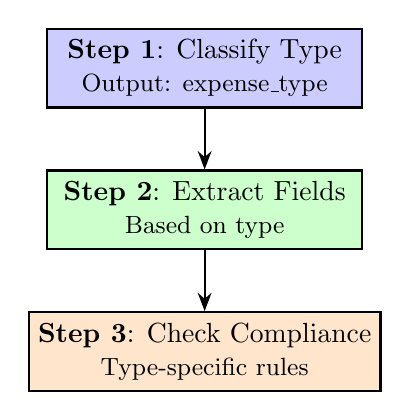
\begin{tikzpicture}[
  box/.style={rectangle, draw, thick, minimum width=4cm, minimum height=1cm, text centered, align=center},
  arrow/.style={->, thick, >=Stealth}
]
  \node[box, fill=blue!20] (classify) at (0,0) {\textbf{Step 1}: Classify Type \\ {\small Output: expense\_type}};
  \node[box, fill=green!20] (extract) at (0,-1.8) {\textbf{Step 2}: Extract Fields \\ {\small Based on type}};
  \node[box, fill=orange!20] (check) at (0,-3.6) {\textbf{Step 3}: Check Compliance \\ {\small Type-specific rules}};

  \draw[arrow] (classify) -- (extract);
  \draw[arrow] (extract) -- (check);
\end{tikzpicture}
\end{center}
\vspace{0.2cm}

\textbf{Key idea}: Each step is simple and has a single responsibility
\end{frame}

\begin{frame}[fragile]{Step 1: Classify Expense Type}
\textbf{First prompt}: Just classify the type
\vspace{0.2cm}

\begin{block}{Classification Prompt}
{\small
Classify this expense into one of three categories:
\begin{itemize}
\item Travel (flights, hotels, conferences, transportation)
\item Office Supplies (equipment, software, books)
\item Meals/Entertainment (restaurants, client dinners)
\end{itemize}

Receipt: [Dinner at restaurant, \$48.50]

Return JSON: \{"expense\_type": "..."\}
}
\end{block}
\vspace{0.2cm}

\textbf{Result}: \texttt{\{"expense\_type": "Meals/Entertainment"\}}
\end{frame}

\begin{frame}[fragile]{Step 2: Conditional Logic in Code}
\textbf{Now we can apply type-specific logic in our code}:
\vspace{0.2cm}

\begin{block}{Python Logic}
{\small
\begin{verbatim}
if expense_type == "Travel":
    # Extract: trip_purpose, destination, dates
    run_travel_prompt()

elif expense_type == "Meals/Entertainment":
    # Extract: attendees, business_purpose
    run_meals_ent_prompt()

elif expense_type == "Office Supplies":
    run_office_supplies_prompt()
\end{verbatim}
}
\end{block}
\vspace{0.2cm}

\textbf{Key insight}: LLMs are great at classification; code is great at conditional logic
\end{frame}

\begin{frame}{Results After Decomposition}
\textbf{What improved}:
\begin{itemize}
    \item Classification is more consistent and reliable
    \item Type-specific rules are explicit in code
    \item Easy to debug (we can inspect the output of each step)
    \item Can test classification independently from validation
\end{itemize}
\vspace{0.3cm}

\textbf{Takeaway}:
\begin{center}
\fcolorbox{blue!80}{blue!10}{%
\begin{minipage}{0.85\textwidth}
\centering
\textbf{Simplify each prompt by breaking complex tasks into stages}

Use LLMs for unstructured→structured transformation

Use code for logic and conditional rules
\end{minipage}
}
\end{center}
\end{frame}

\section{Iteration 2: Grounding with Citations}

\begin{frame}{New Problem: Hallucination}
\textbf{Context}: We're checking for prohibited expenses (alcohol)
\vspace{0.2cm}

\textbf{Prompt}:
{\small
Does this receipt contain alcohol? Return JSON: \{"contains\_alcohol": true/false, "reason": "..."\}

Receipt: [Restaurant bill, \$48.50, two entrees and soft drinks]
}
\vspace{0.3cm}

\textbf{Result}:
{\small \texttt{\{"contains\_alcohol": true, "reason": "Likely includes wine or beer with dinner"\}}}
\vspace{0.3cm}

\textbf{Problem}: The model \textit{assumed} there was alcohol when the receipt never mentioned it!
\end{frame}

\begin{frame}{Why This Happens}
\textbf{LLMs are pattern matchers}, not database lookups:
\begin{itemize}
    \item Restaurant + dinner → often includes alcohol in training data
    \item Model generates "plausible" answers based on patterns
    \item Without explicit evidence requirement, it fills in gaps
\end{itemize}
\vspace{0.3cm}

\textbf{This is dangerous}:
\begin{itemize}
    \item False rejections (denying valid expenses)
    \item Compliance issues (wrong reasons in audit trail)
    \item Loss of trust in the system
\end{itemize}
\end{frame}

\begin{frame}[fragile]{Solution: Require Citations}
\textbf{Better prompt}: Demand evidence from the receipt or ask to verify before returning (which can add \$\$\$)
\vspace{0.2cm}

\begin{block}{Grounded Prompt}
{\small
Does this receipt contain alcohol?

\textbf{You MUST cite exact quotes from the receipt to support your answer.}

If alcohol is present, provide the exact line items that mention it.

Receipt: [Restaurant bill, \$48.50, two entrees and soft drinks]

Return JSON:
\begin{verbatim}
{
  "contains_alcohol": true/false,
  "evidence": ["exact quote 1", "exact quote 2"],
  "reason": "explanation based on evidence"
}
\end{verbatim}
}
\end{block}
\end{frame}

\begin{frame}[fragile]{Results After Grounding}
\textbf{New result}:
{\small
\begin{verbatim}
{
  "contains_alcohol": false,
  "evidence": [],
  "reason": "No alcohol items found in receipt.
            Items listed: 2x Lunch Special, 2x Soft Drink"
}
\end{verbatim}
}
\vspace{0.3cm}

\textbf{What improved}:
\begin{itemize}
    \item Model is forced to ground claims in actual receipt text
    \item Hallucinations are reduced significantly
    \item We get an audit trail (can verify the evidence ourselves)
    \item False positives drop dramatically
\end{itemize}
\end{frame}

\begin{frame}{Grounding Best Practices}
\textbf{How to apply grounding}:
\begin{enumerate}
    \item Require exact quotes or citations for any factual claims
    \item Ask for evidence \textit{before} conclusions
    \item Validate that evidence exists in the source material
    \item Use structured output with separate "evidence" field
\end{enumerate}
\vspace{0.3cm}

\textbf{When to use it}:
\begin{itemize}
    \item Compliance/regulatory contexts (must justify decisions)
    \item Extracting facts from documents
    \item Any scenario where hallucination is risky
\end{itemize}
\vspace{0.3cm}

\begin{center}
\fcolorbox{green!80}{green!10}{%
\begin{minipage}{0.85\textwidth}
\centering
\textbf{Citations turn the LLM from a "creative writer" into an "evidence-based analyst"}
\end{minipage}
}
\end{center}
\end{frame}

\section{Iteration 3: Few-Shot Examples}

\begin{frame}{Another Problem: Edge Cases}
\textbf{Context}: Classification works well for obvious cases
\vspace{0.3cm}

\textbf{But what about ambiguous expenses?}
\begin{itemize}
    \item Conference registration: Travel or Office Supplies?
    \item Team building dinner: Meals or Office Supplies?
    \item Online course subscription: Office Supplies or ???
    \item Software for a specific project: Office Supplies or ???
\end{itemize}
\vspace{0.3cm}

\textbf{Problem}: Model makes inconsistent decisions on edge cases
\begin{itemize}
    \item Conference registration sometimes classified as "Office Supplies"
    \item No clear policy guidance in the prompt
\end{itemize}
\end{frame}

\begin{frame}[fragile]{Solution: Provide Examples}
\textbf{Better prompt}: Show the model what good classification looks like
\vspace{0.2cm}

\begin{block}{Few-Shot Prompt}
{\small
Classify this expense. Here are some examples:

\textbf{Example 1}:
Receipt: Conference registration, AI Summit 2024, \$500
Classification: Travel (conferences are travel-related)

\textbf{Example 2}:
Receipt: Office chair from Staples, \$200
Classification: Office Supplies (furniture and equipment)

\textbf{Example 3}:
Receipt: Team dinner at local restaurant, \$120
Classification: Meals/Entertainment (company-sponsored meals)

Now classify:
Receipt: [Your receipt here]
}
\end{block}
\end{frame}

\begin{frame}{Types of Examples to Include}
\textbf{Good few-shot examples include}:
\begin{enumerate}
    \item \textbf{Positive examples}: Correct classifications
    \item \textbf{Edge cases}: Ambiguous situations with your preferred handling
    \item \textbf{Negative examples}: Common mistakes to avoid
\end{enumerate}
\vspace{0.3cm}

\textbf{Example - Negative case}:
{\small
Receipt: Laptop purchased for work, \$1,200

\textit{Incorrect}: Meals/Entertainment

\textit{Correct}: Office Supplies (technology equipment)

\textit{Reason}: Even though expensive, hardware is office supplies, not travel
}
\vspace{0.3cm}

\textbf{How many examples?} 2-5 is usually enough; more isn't always better
\end{frame}

\begin{frame}{Results After Few-Shot Examples}
\textbf{What improved}:
\begin{itemize}
    \item Edge cases are now handled consistently
    \item Model learns your organization's specific policies
    \item Classification accuracy improves on ambiguous cases
    \item Fewer surprises and unexpected categorizations
\end{itemize}
\vspace{0.3cm}

\textbf{Tradeoff}:
\begin{itemize}
    \item More tokens in prompt (costs more, takes longer)
    \item Need to maintain example set
    \item But: much more reliable results
\end{itemize}
\vspace{0.3cm}

\begin{center}
\fcolorbox{orange!80}{orange!10}{%
\begin{minipage}{0.85\textwidth}
\centering
\textbf{Examples teach the model your specific policies and edge case handling}
\end{minipage}
}
\end{center}
\end{frame}

\section{Other Techniques}

\begin{frame}{Additional Performance Techniques}
\textbf{Beyond decomposition, grounding, and examples}:
\vspace{0.3cm}

\begin{enumerate}
    \item \textbf{Role/Persona Specification}
    \begin{itemize}
        \item "You are a careful compliance officer reviewing expenses..."
        \item Sets tone and behavior expectations
    \end{itemize}

    \item \textbf{Providing Domain Context}
    \begin{itemize}
        \item Include relevant company policies in the prompt
        \item Specific rules and thresholds from your domain
    \end{itemize}

    \item \textbf{Adding Guardrails}
    \begin{itemize}
        \item Structured output schemas (JSON with required fields)
        \item Validation logic to catch impossible outputs
        \item Allowed/blocked lists (e.g., only these 3 expense types)
    \end{itemize}
\end{enumerate}
\end{frame}

\begin{frame}{More Advanced Techniques}
\begin{enumerate}
    \setcounter{enumi}{3}
    \item \textbf{Chain-of-Thought Prompting}
    \begin{itemize}
        \item Ask model to "show your reasoning step by step"
        \item Improves accuracy on complex logic problems
        \item Makes debugging easier
    \end{itemize}

    \item \textbf{Temperature Tuning}
    \begin{itemize}
        \item Lower temperature (0.0-0.3) for consistency
        \item Higher temperature (0.7-1.0) for creativity
        \item Classification and extraction: use low temperature
    \end{itemize}

    \item \textbf{Output Validation}
    \begin{itemize}
        \item Check LLM outputs with deterministic code
        \item Re-prompt if validation fails
        \item Combine AI flexibility with code reliability
    \end{itemize}
\end{enumerate}
\end{frame}

\begin{frame}{The Three Core Techniques (Summary)}
\begin{center}
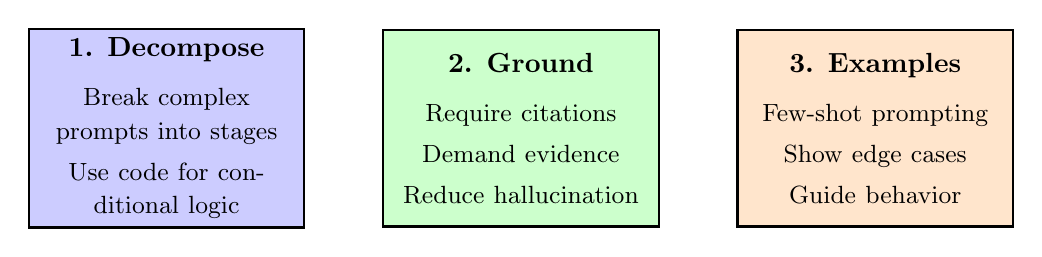
\begin{tikzpicture}[
  box/.style={rectangle, draw, thick, minimum width=3.5cm, minimum height=2.5cm, text width=3.2cm, align=center},
]
  \node[box, fill=blue!20] (decompose) at (0,0) {
    \textbf{1. Decompose}\\[0.2cm]
    {\small Break complex prompts into stages}\\[0.1cm]
    {\small Use code for conditional logic}
  };

  \node[box, fill=green!20] (ground) at (4.5,0) {
    \textbf{2. Ground}\\[0.2cm]
    {\small Require citations}\\[0.1cm]
    {\small Demand evidence}\\[0.1cm]
    {\small Reduce hallucination}
  };

  \node[box, fill=orange!20] (examples) at (9,0) {
    \textbf{3. Examples}\\[0.2cm]
    {\small Few-shot prompting}\\[0.1cm]
    {\small Show edge cases}\\[0.1cm]
    {\small Guide behavior}
  };
\end{tikzpicture}
\end{center}
\vspace{0.5cm}

\textbf{Use these in combination for best results}
\end{frame}

\section{Your Turn: Improving the Resume Scorer}

\begin{frame}{Today's Workflow}
\textbf{You will work with 3 randomly sampled resumes}:
\begin{enumerate}
    \item \textbf{Baseline}: Run the monolithic scorer
    \begin{itemize}
        \item Single prompt: resume → 0-100 score
        \item Collect results in a DataFrame
    \end{itemize}
    \vspace{0.2cm}

    \item \textbf{TODO 1}: Extract years of experience
    \begin{itemize}
        \item Write a focused prompt to extract only years of experience
        \item Require citations/evidence from resume
        \item Run on all 3 samples, create DataFrame
    \end{itemize}
    \vspace{0.2cm}

    \item \textbf{TODO 2}: Extract and score technologies
    \begin{itemize}
        \item Extract technologies/skills from resume
        \item Compare against required technologies in job req
        \item Score 0-100 based on match percentage
    \end{itemize}
\end{enumerate}
\end{frame}

\begin{frame}{Today's Workflow (continued)}
\begin{enumerate}
    \setcounter{enumi}{3}
    \item \textbf{TODO 3}: Combine and compare
    \begin{itemize}
        \item Merge year data with technology scores
        \item Create a composite score from extracted features
        \item Compare against monolithic 0-100 scores
        \item Analyze: Which is more consistent? Which explains better?
    \end{itemize}
    \vspace{0.2cm}

    \item \textbf{TODO 4}: Extensions (pick one or more)
    \begin{itemize}
        \item Education requirements extraction
        \item Leadership/mentoring experience
        \item Scale to 20 resumes and compare costs
    \end{itemize}
\end{enumerate}
\end{frame}

\begin{frame}{Key Takeaways for Your Work}
\textbf{Apply the three core techniques}:
\begin{itemize}
    \item \textbf{Decomposition}: Break scoring into feature extraction steps
    \item \textbf{Grounding}: Require citations for years of experience
    \item \textbf{Examples}: (Optional) Add few-shot examples for edge cases
\end{itemize}
\vspace{0.3cm}

\textbf{What to look for}:
\begin{itemize}
    \item Are decomposed scores more explainable than monolithic scores?
    \item Can you justify each score with specific extracted features?
    \item How do token costs compare between approaches?
    \item Which approach would you trust more in production?
\end{itemize}
\vspace{0.3cm}

\end{frame}

\begin{frame}{Let's Get Started!}
\begin{center}
\Large
Open the notebook: \\[0.3cm]
\texttt{lecture\_3\_resume\_scorer\_improvement.ipynb}
\\[1cm]

Work through TODOs 1-4 \\[0.3cm]
Compare your results \\[0.3cm]
Discuss with your team
\end{center}
\end{frame}

\end{document}
